
%%%%%%%%%%%%%%%%%%%%%%%%%%%%%%%%%%%%%%%%%%%%%%%%%%%%%%%%%%%%%%%%%%%%%
%% This is a (brief) model paper using the achemso class
%% The document class accepts keyval options, which should include
%% the target journal and optionally the manuscript type.
%%%%%%%%%%%%%%%%%%%%%%%%%%%%%%%%%%%%%%%%%%%%%%%%%%%%%%%%%%%%%%%%%%%%%
\documentclass[journal=acscii,manuscript=article]{achemso}

%%%%%%%%%%%%%%%%%%%%%%%%%%%%%%%%%%%%%%%%%%%%%%%%%%%%%%%%%%%%%%%%%%%%%
%% Place any additional packages needed here.  Only include packages
%% which are essential, to avoid problems later. Do NOT use any
%% packages which require e-TeX (for example etoolbox): the e-TeX
%% extensions are not currently available on the ACS conversion
%% servers.
%%%%%%%%%%%%%%%%%%%%%%%%%%%%%%%%%%%%%%%%%%%%%%%%%%%%%%%%%%%%%%%%%%%%%
\usepackage[version=3]{mhchem} % Formula subscripts using \ce{}
\usepackage[T1]{fontenc}       % Use modern font encodings
\usepackage{lineno}
\linenumbers

\usepackage{epstopdf}
\usepackage[utf8]{inputenc} % allow utf-8 input
% \usepackage[T1]{fontenc}    % use 8-bit T1 fonts
\usepackage{hyperref}       % hyperlinks
\usepackage{url}            % simple URL typesetting
\usepackage{booktabs}       % professional-quality tables
\usepackage{amsfonts}       % blackboard math symbols
\usepackage{microtype}      % microtypography
\usepackage{graphicx}
\usepackage[subrefformat=parens,labelformat=parens]{subcaption}
\usepackage{algorithm}
\usepackage[noend]{algpseudocode}
\usepackage{hyperref}
\usepackage{color,soul}
\usepackage{amsmath,amsthm,amssymb,amsfonts}
\usepackage{mathtools}
\mathtoolsset{showonlyrefs}
\usepackage{placeins}

%\graphicspath{{../}}

%%%%%%%%%%%%%%%%%%%%%%%%%%%%%%%%%%%%%%%%%%%%%%%%%%%%%%%%%%%%%%%%%%%%%
%% If issues arise when submitting your manuscript, you may want to
%% un-comment the next line.  This provides information on the
%% version of every file you have used.
%%%%%%%%%%%%%%%%%%%%%%%%%%%%%%%%%%%%%%%%%%%%%%%%%%%%%%%%%%%%%%%%%%%%%
%%\listfiles

%%%%%%%%%%%%%%%%%%%%%%%%%%%%%%%%%%%%%%%%%%%%%%%%%%%%%%%%%%%%%%%%%%%%%
%% Place any additional macros here.  Please use \newcommand* where
%% possible, and avoid layout-changing macros (which are not used
%% when typesetting).
%%%%%%%%%%%%%%%%%%%%%%%%%%%%%%%%%%%%%%%%%%%%%%%%%%%%%%%%%%%%%%%%%%%%%
\newcommand*\mycommand[1]{\texttt{\emph{#1}}}
\newcommand{\sidecaption}[1]% #1 = label name
{\raisebox{\abovecaptionskip}{\begin{subfigure}[t]{1.6em}
  \caption[singlelinecheck=off]{}% do not center
  \label{#1}
\end{subfigure}}\ignorespaces}

\algrenewcommand{\algorithmicrequire}{\textbf{Input:}}
\algrenewcommand{\algorithmicensure}{\textbf{Output:}}
\algrenewcommand\Return{\State\algorithmicreturn{}~}
\algrenewcommand\algorithmicindent{1.0em}%


%%%%%%%%%%%%%%%%%%%%%%%%%%%%%%%%%%%%%%%%%%%%%%%%%%%%%%%%%%%%%%%%%%%%%
%% Meta-data block
%% ---------------
%% Each author should be given as a separate \author command.
%%
%% Corresponding authors should have an e-mail given after the author
%% name as an \email command. Phone and fax numbers can be given
%% using \phone and \fax, respectively; this information is optional.
%%
%% The affiliation of authors is given after the authors; each
%% \affiliation command applies to all preceding authors not already
%% assigned an affiliation.
%%
%% The affiliation takes an option argument for the short name.  This
%% will typically be something like "University of Somewhere".
%%
%% The \altaffiliation macro should be used for new address, etc.
%% On the other hand, \alsoaffiliation is used on a per author basis
%% when authors are associated with multiple institutions.
%%%%%%%%%%%%%%%%%%%%%%%%%%%%%%%%%%%%%%%%%%%%%%%%%%%%%%%%%%%%%%%%%%%%%



\author{Rafael G\'omez-Bombarelli}
\affiliation{Kyulux North America Inc., 10 Post Office Sq., Suite 800, Boston, MA 02109, USA}
\altaffiliation{Equal contribution}

\author{Jennifer N. Wei}
\affiliation{Department of Chemistry and Chemical Biology, Harvard University, Cambridge MA 02138, USA}
\altaffiliation{Equal contribution}

\author{David Duvenaud}
\affiliation{Department of Computer Science, University of Toronto}
\altaffiliation{Equal contribution}

\author{Jos\'e Miguel Hern\'andez-Lobato}
\affiliation{Department of Engineering, University of Cambridge Trumpington Street, Cambridge CB2 1PZ, UK}
\altaffiliation{Equal contribution}

\author{Benjam\'in S\'anchez-Lengeling}
\author{Dennis Sheberla}
\affiliation{Department of Chemistry and Chemical Biology, Harvard University, Cambridge MA 02138, USA}

\author{Jorge Aguilera-Iparraguirre}
\affiliation{Kyulux North America Inc., 10 Post Office Sq., Suite 800, Boston, MA 02109, USA}

\author{Timothy D. Hirzel}
\affiliation{Kyulux North America Inc., 10 Post Office Sq., Suite 800, Boston, MA 02109, USA}

\author{Ryan P. Adams}
\affiliation{Google Brain and Princeton University}

\author{Al\'an Aspuru-Guzik}
\email{aspuru@chemistry.harvard.edu}
\affiliation{Department of Chemistry and Chemical Biology, Harvard University, Cambridge MA 02138, USA}
\alsoaffiliation{Canadian Institute for Advanced Research (CIFAR), Biologically-Inspired Solar Energy Program.}

\title{Supporting Information for Automatic Chemical Design Using a Data-Driven Continuous Representation of Molecules} 

\begin{document}


\begin{table}[h]
\centering
\begin{tabular}{|c|c|c|}
\hline 
Dataset & ZINC & QM \\ 
\hline 
Training set & 92.1 & 99.6 \\ 
\hline 
Test set & 90.7 & 99.4 \\ 
\hline 
ZINC & 91.0 & 1.4 \\ 
\hline 
eMolecules & 83.8 & 8.8 \\ 
\hline 
\end{tabular} 
\caption{Percentage of successfully decoding of latent representation after 1000 attempts for 1000 molecules from the traning set, 1000 validation molecules randomly chosen from ZINC and a 1000 validation molecules randomly chosen from eMolecules. Both VAEs perform very well for training data, and they are well transferable within molecules of the same class outside the training data, as evidence by the good validation performance of the ZINC VAE and the underperformance of the QM9 VAE against real-life small molecules.}
\label{tab:recovery statistics}
\end{table}[h]

\begin{table}[h]
\centering
\begin{tabular}{|c|c|c|}
\hline 
Dataset & ZINC & QM \\ 
\hline 
Decoding probability & 73.9 & 79.3 \\  
\hline 
\end{tabular} 
\caption{Percentage of 5000 randomly-selected latent points that decode to valid molecules after 1000 attempts}
\label{tab:random_sampling_statistics}
\end{table}


\begin{table}[h]
\centering
\begin{tabular}{|c|c|c|c|}
\hline 
Training set size &  Categorical Accuracy & logP MAE & QED MAE\\ 
\hline 
225,000 & 99.3\% & 0.15 & 0.054 \\ 
\hline 
175,000 & 99.0\% & 0.18 & 0.076 \\ 
\hline 
125,000 & 98.5\% & 0.15 & 0.076 \\ 
\hline 
25,000 & 91.6\% & 0.23 & 0.079 \\ 
\hline 
\end{tabular} 
\caption{ Variational autoencoder performance over different sizes of datasets. Training and tests were performed using randomly selected molecules from the ZINC dataset, the values reported here are the scores from the validation set. The categorical accuracy reflects the percentage of characters in the output SMILES that were accurately reconstructed. Mean Absolute Errors (MAE) are reported for QED and logP properties. Performance significantly decreases if only ~$10^5$ molecules are used for training.}
\label{tab:Accuracy_by_training_size}
\end{table}




\begin{figure}[h]
\centering
\sidecaption{subfig:a}
\raisebox{-\height}{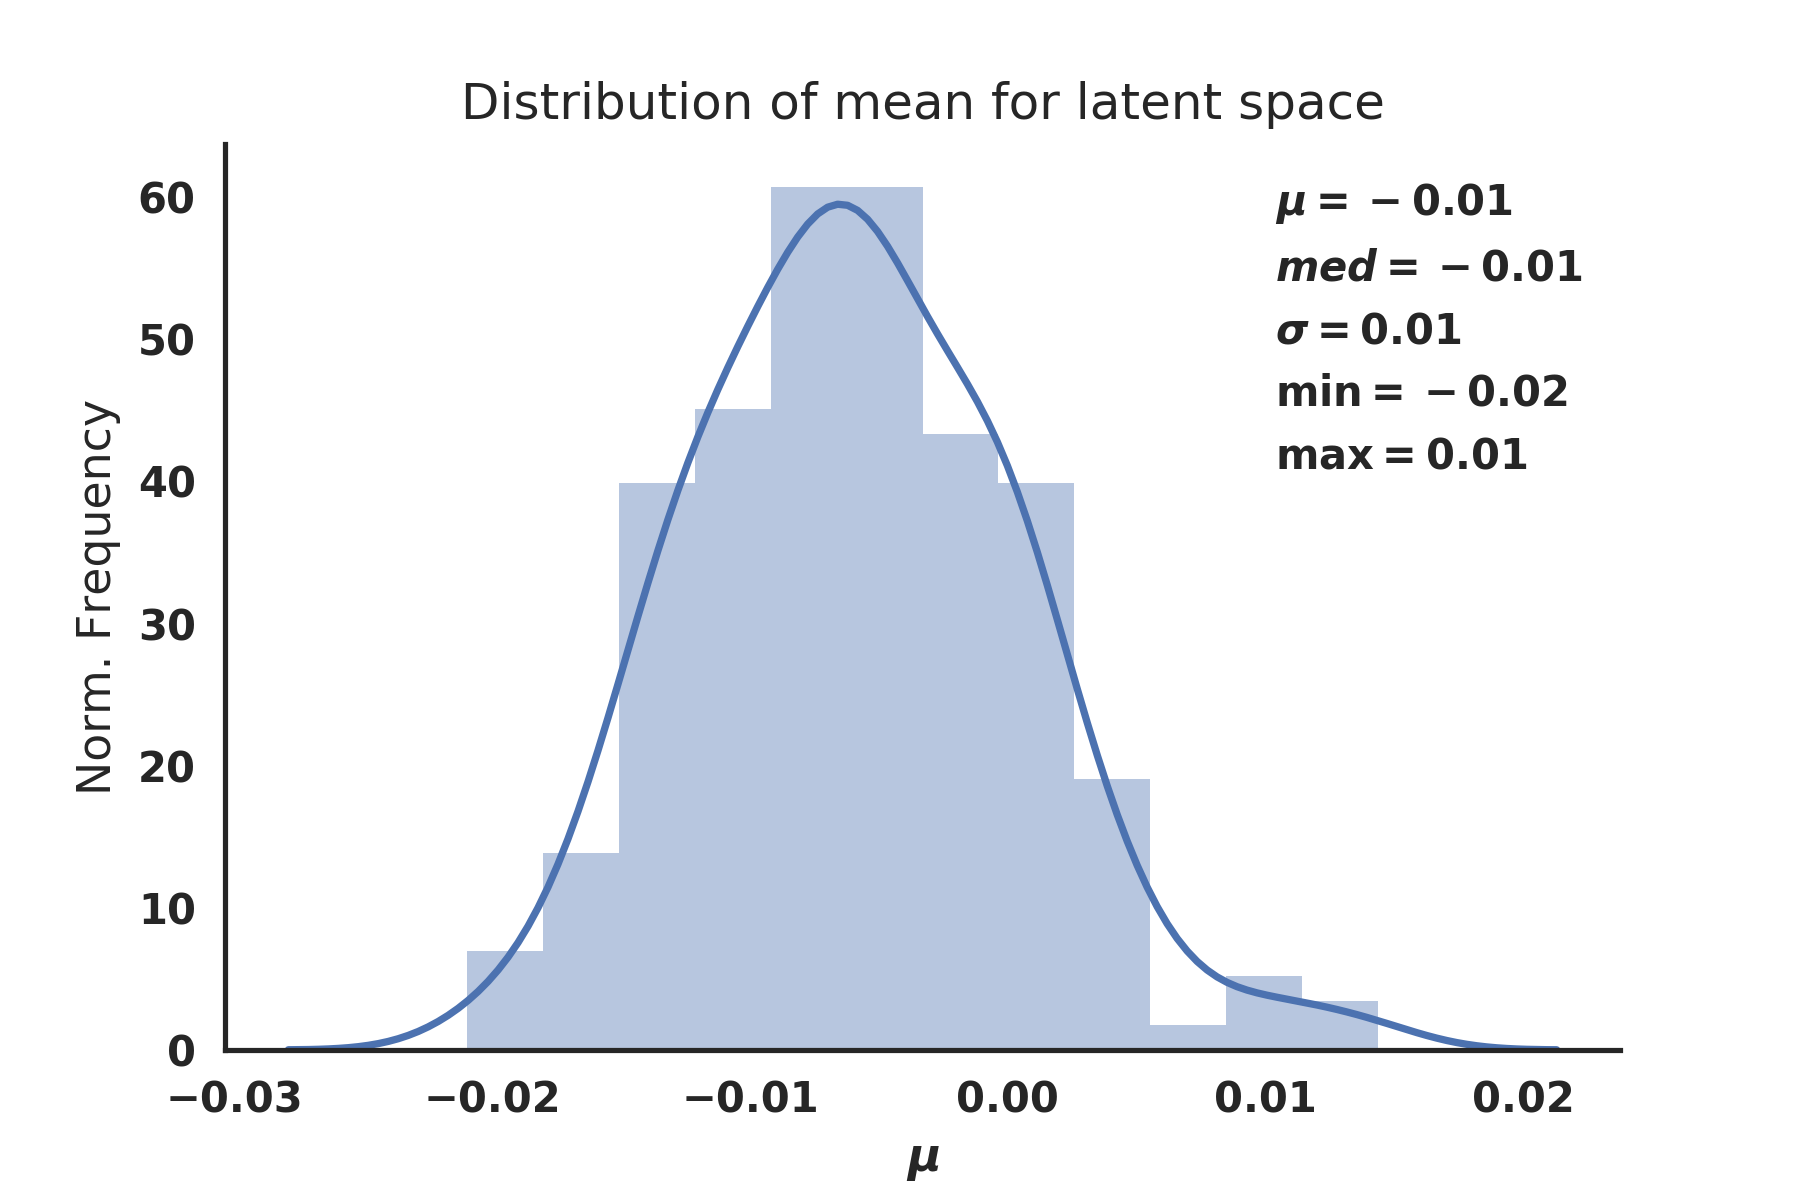
\includegraphics[width=0.45\columnwidth]{figures/mean_Z}}
\sidecaption{subfig:b}
\raisebox{-\height}{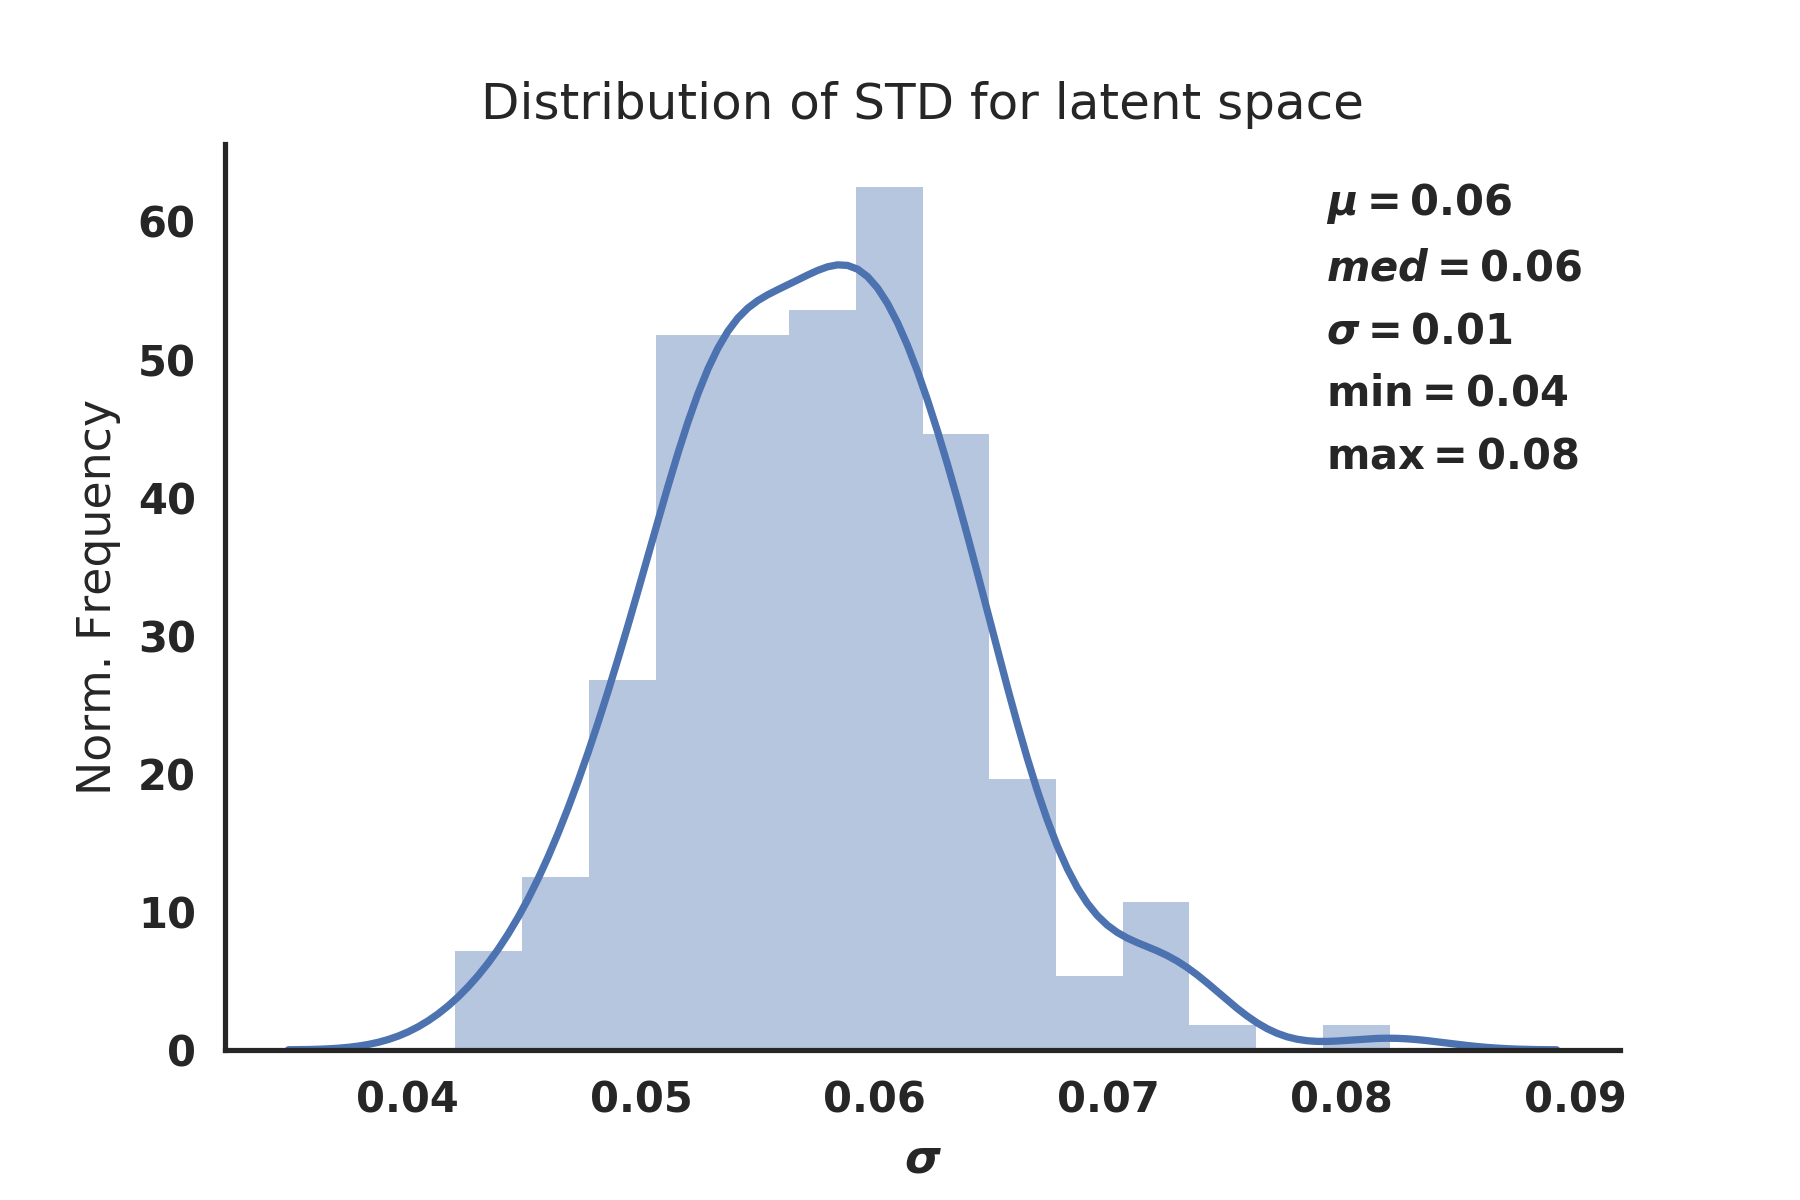
\includegraphics[width=0.45\columnwidth]{figures/STD_Z}}

\sidecaption{subfig:c}
\raisebox{-\height}{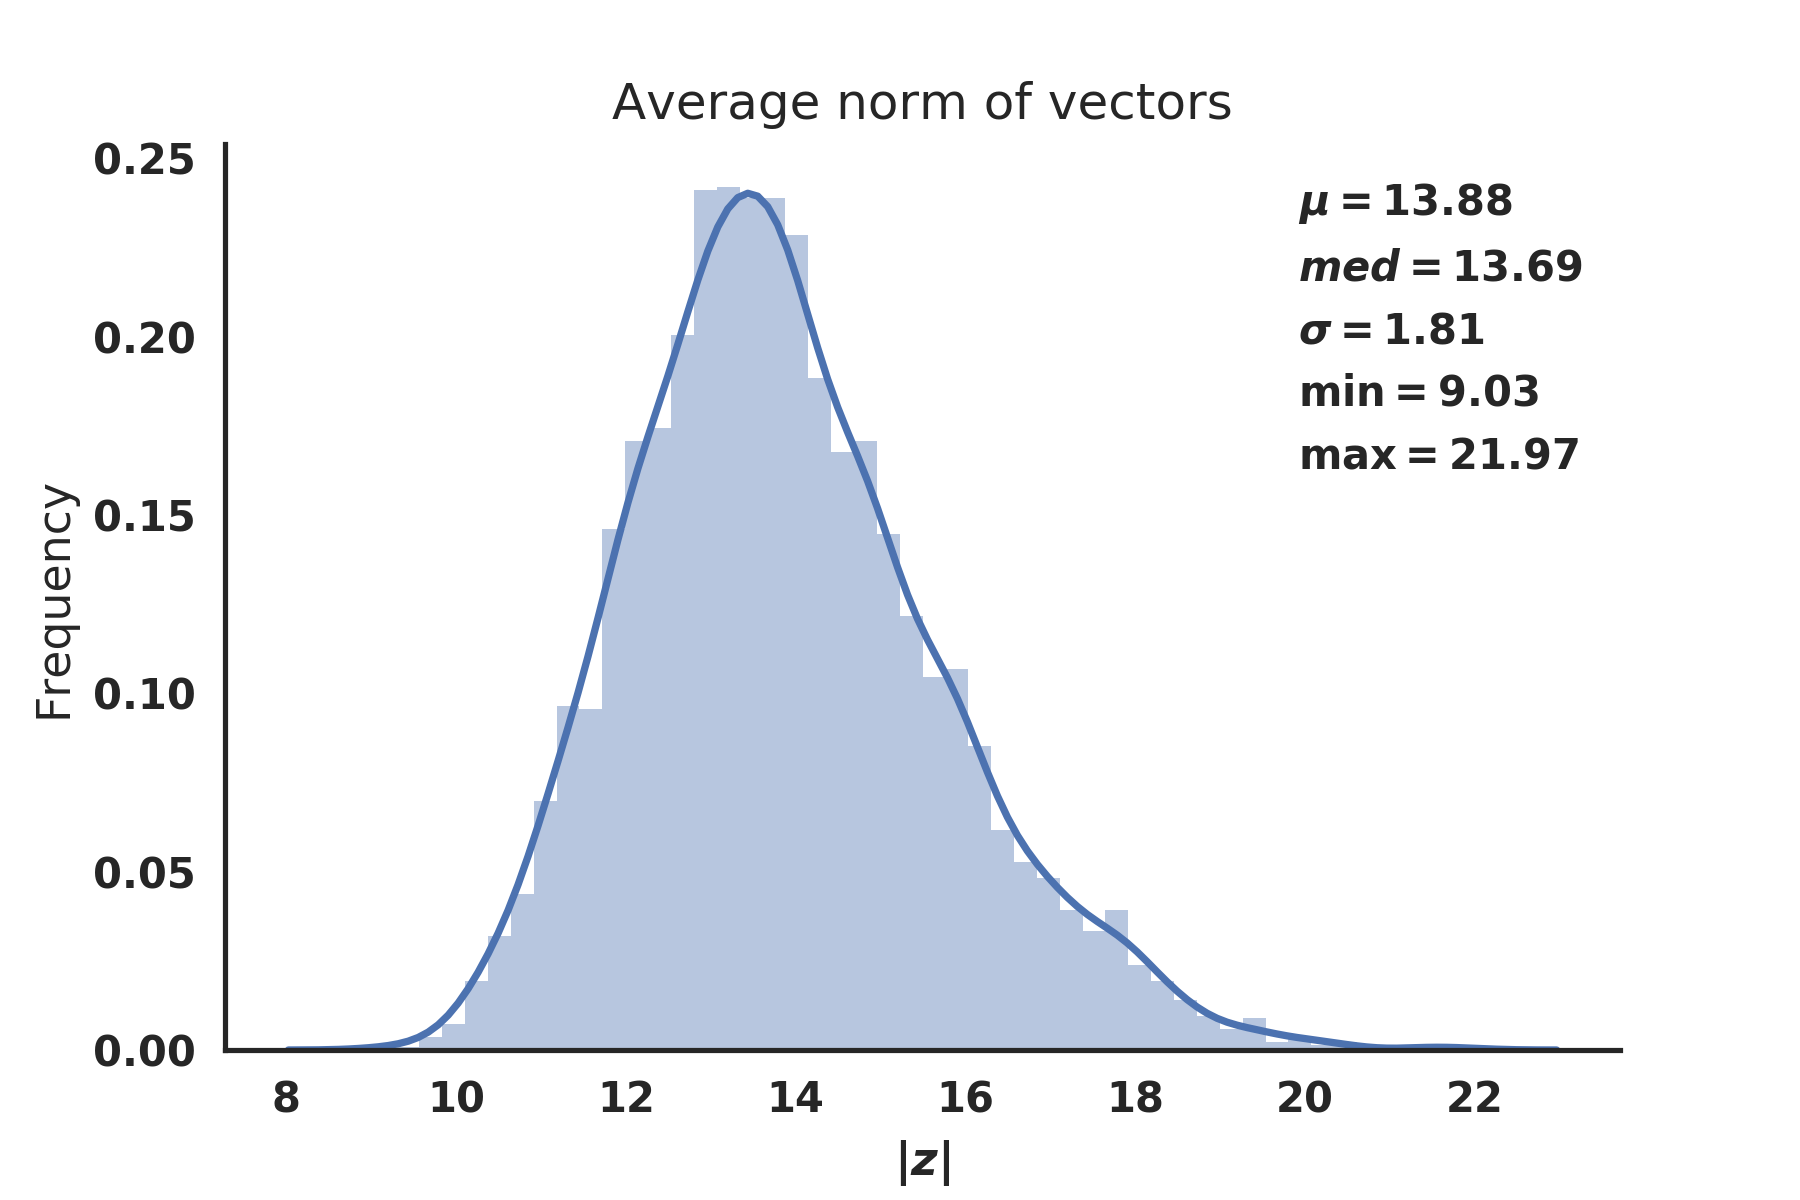
\includegraphics[width=0.45\columnwidth]{figures/norm_Z}}
\sidecaption{subfig:d}
\raisebox{-\height}{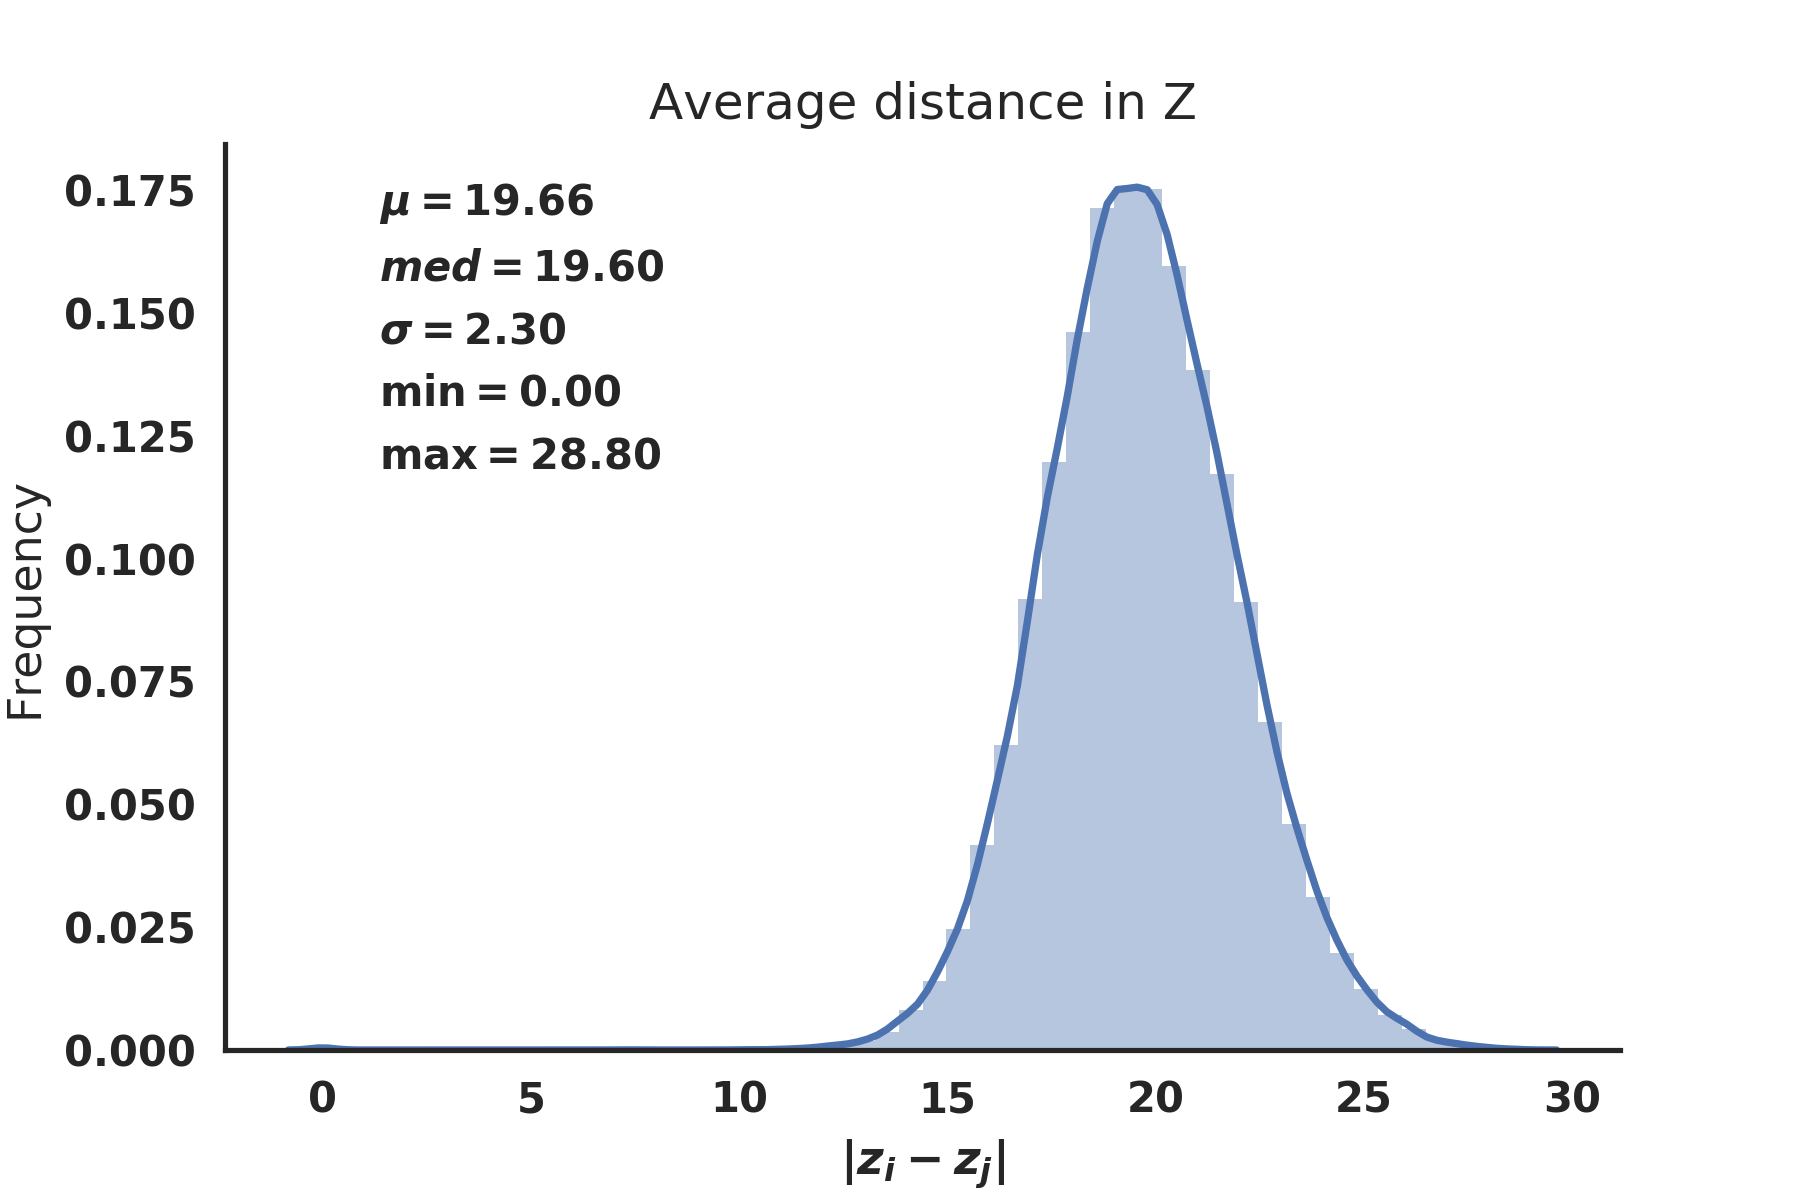
\includegraphics[width=0.45\columnwidth]{figures/distance_Z}}
\caption{Distribution and statistics of (a) the mean of latent space coordinates (b) standard deviation of latent space coordinates (c) norm of latent space coordinates of the encoded representation of randomly selected molecules from the ZINC validation set. (d) Distribution of Euclidean distances between random pairs of validation molecules in the ZINC VAE }
\label{fig:ls_stats}
\end{figure}


\begin{figure}
\centering
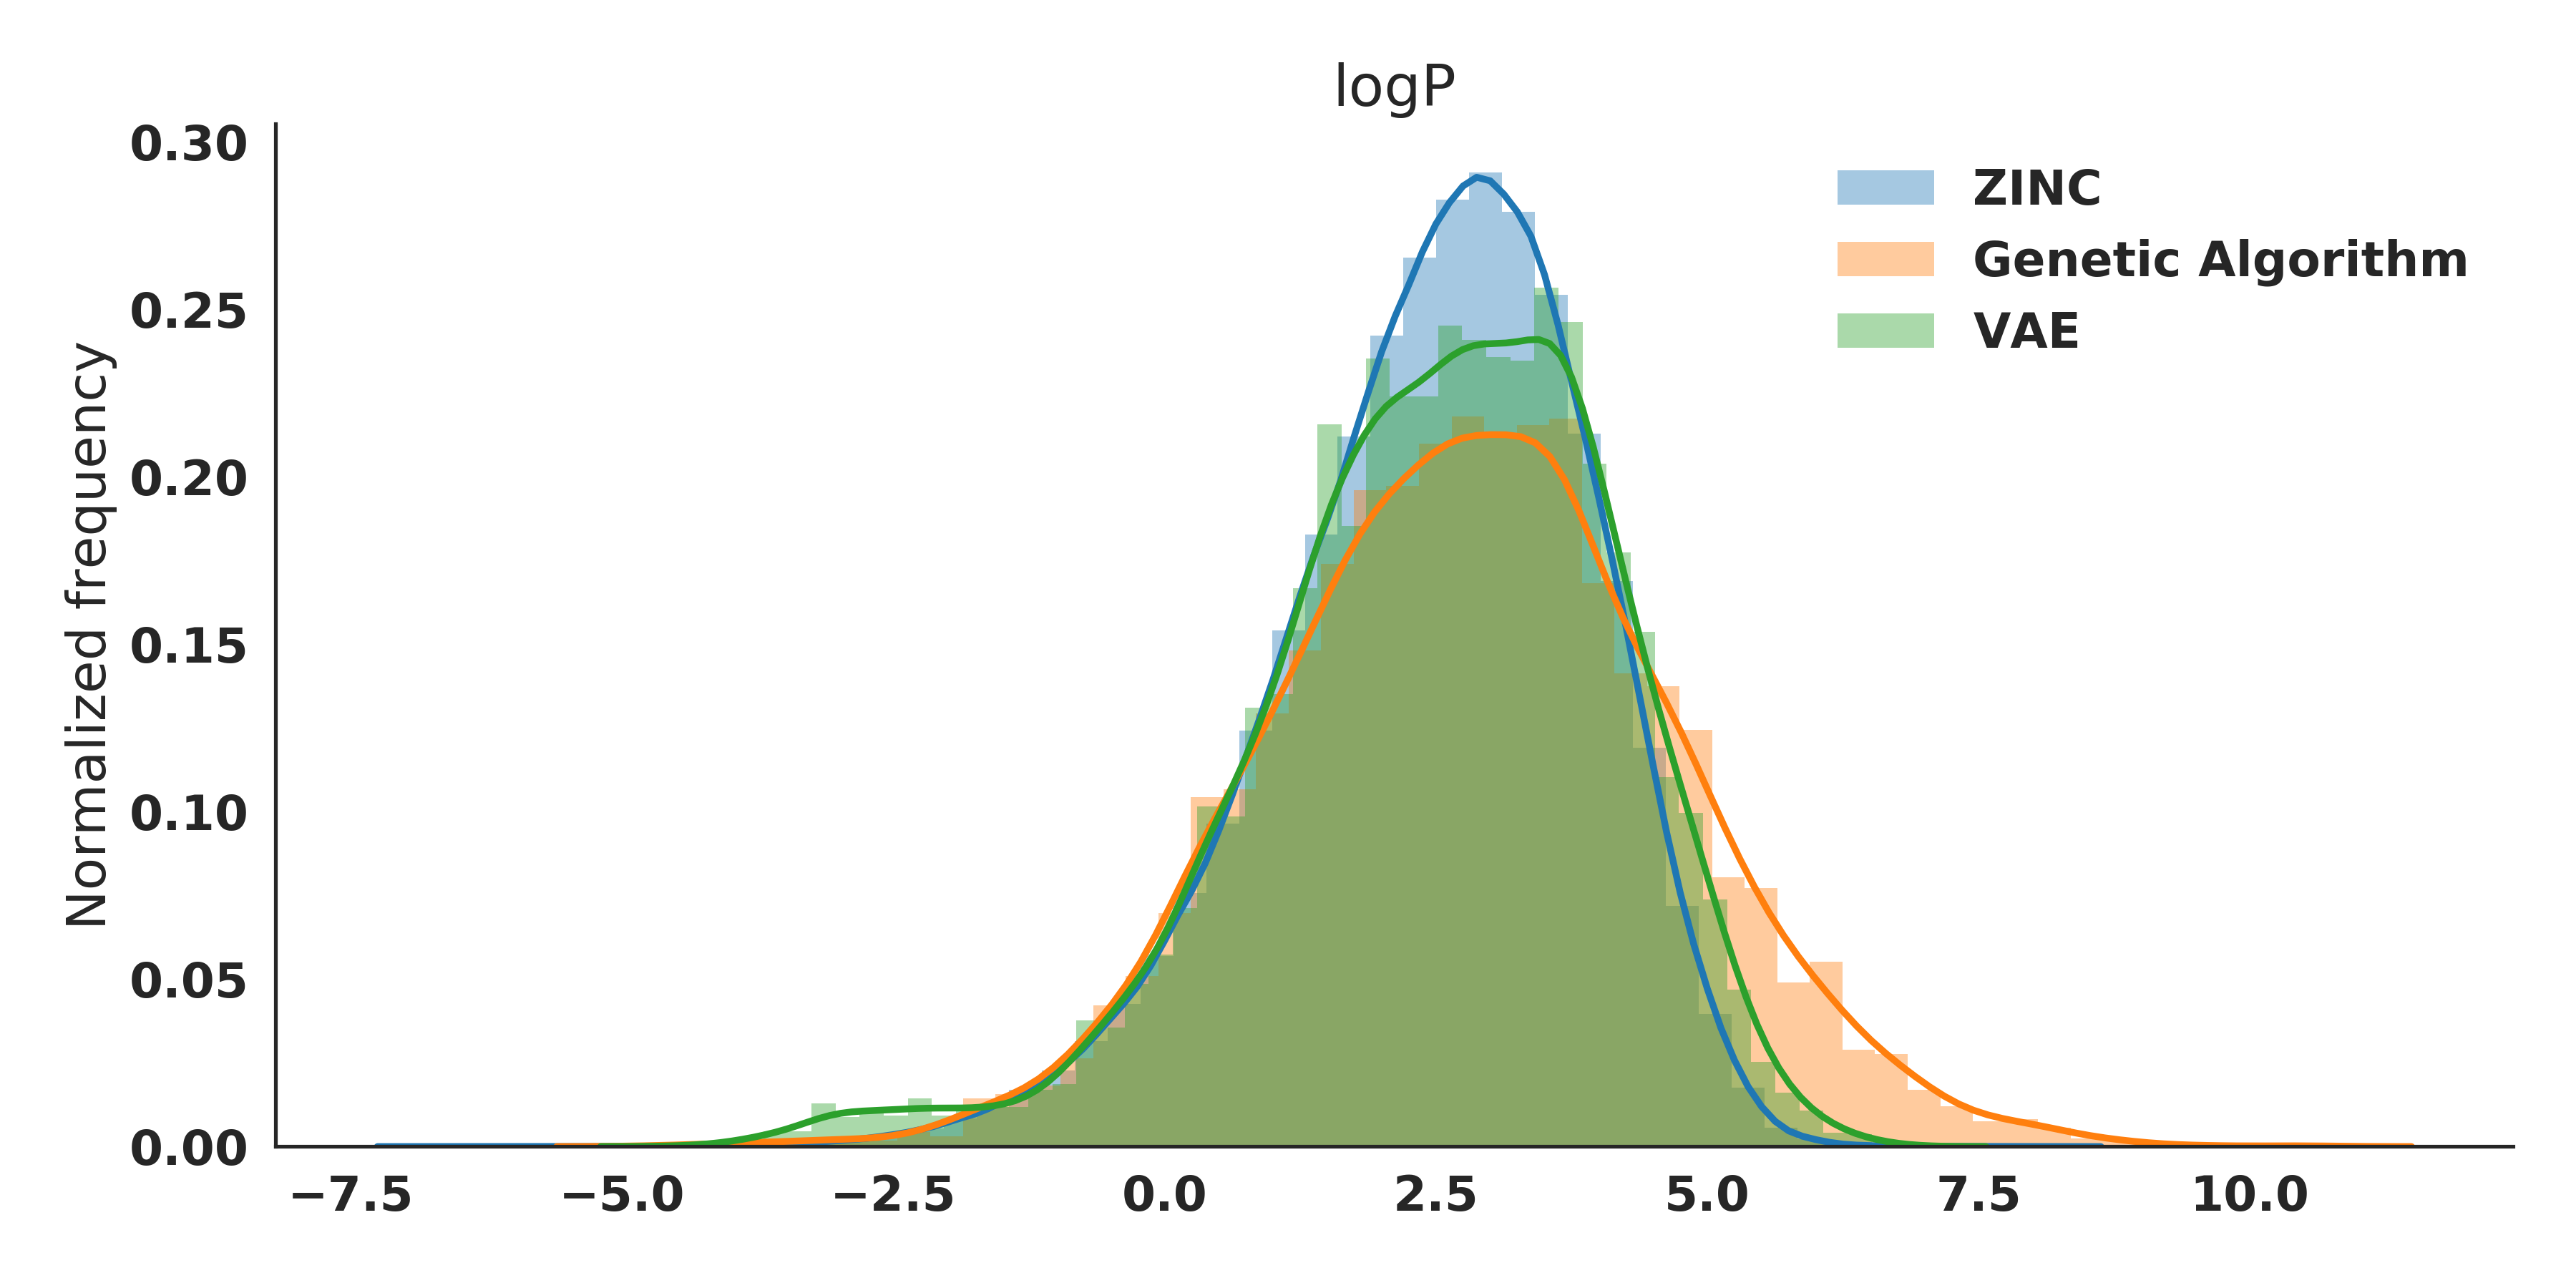
\includegraphics[width=0.3\columnwidth]{figures/logP}
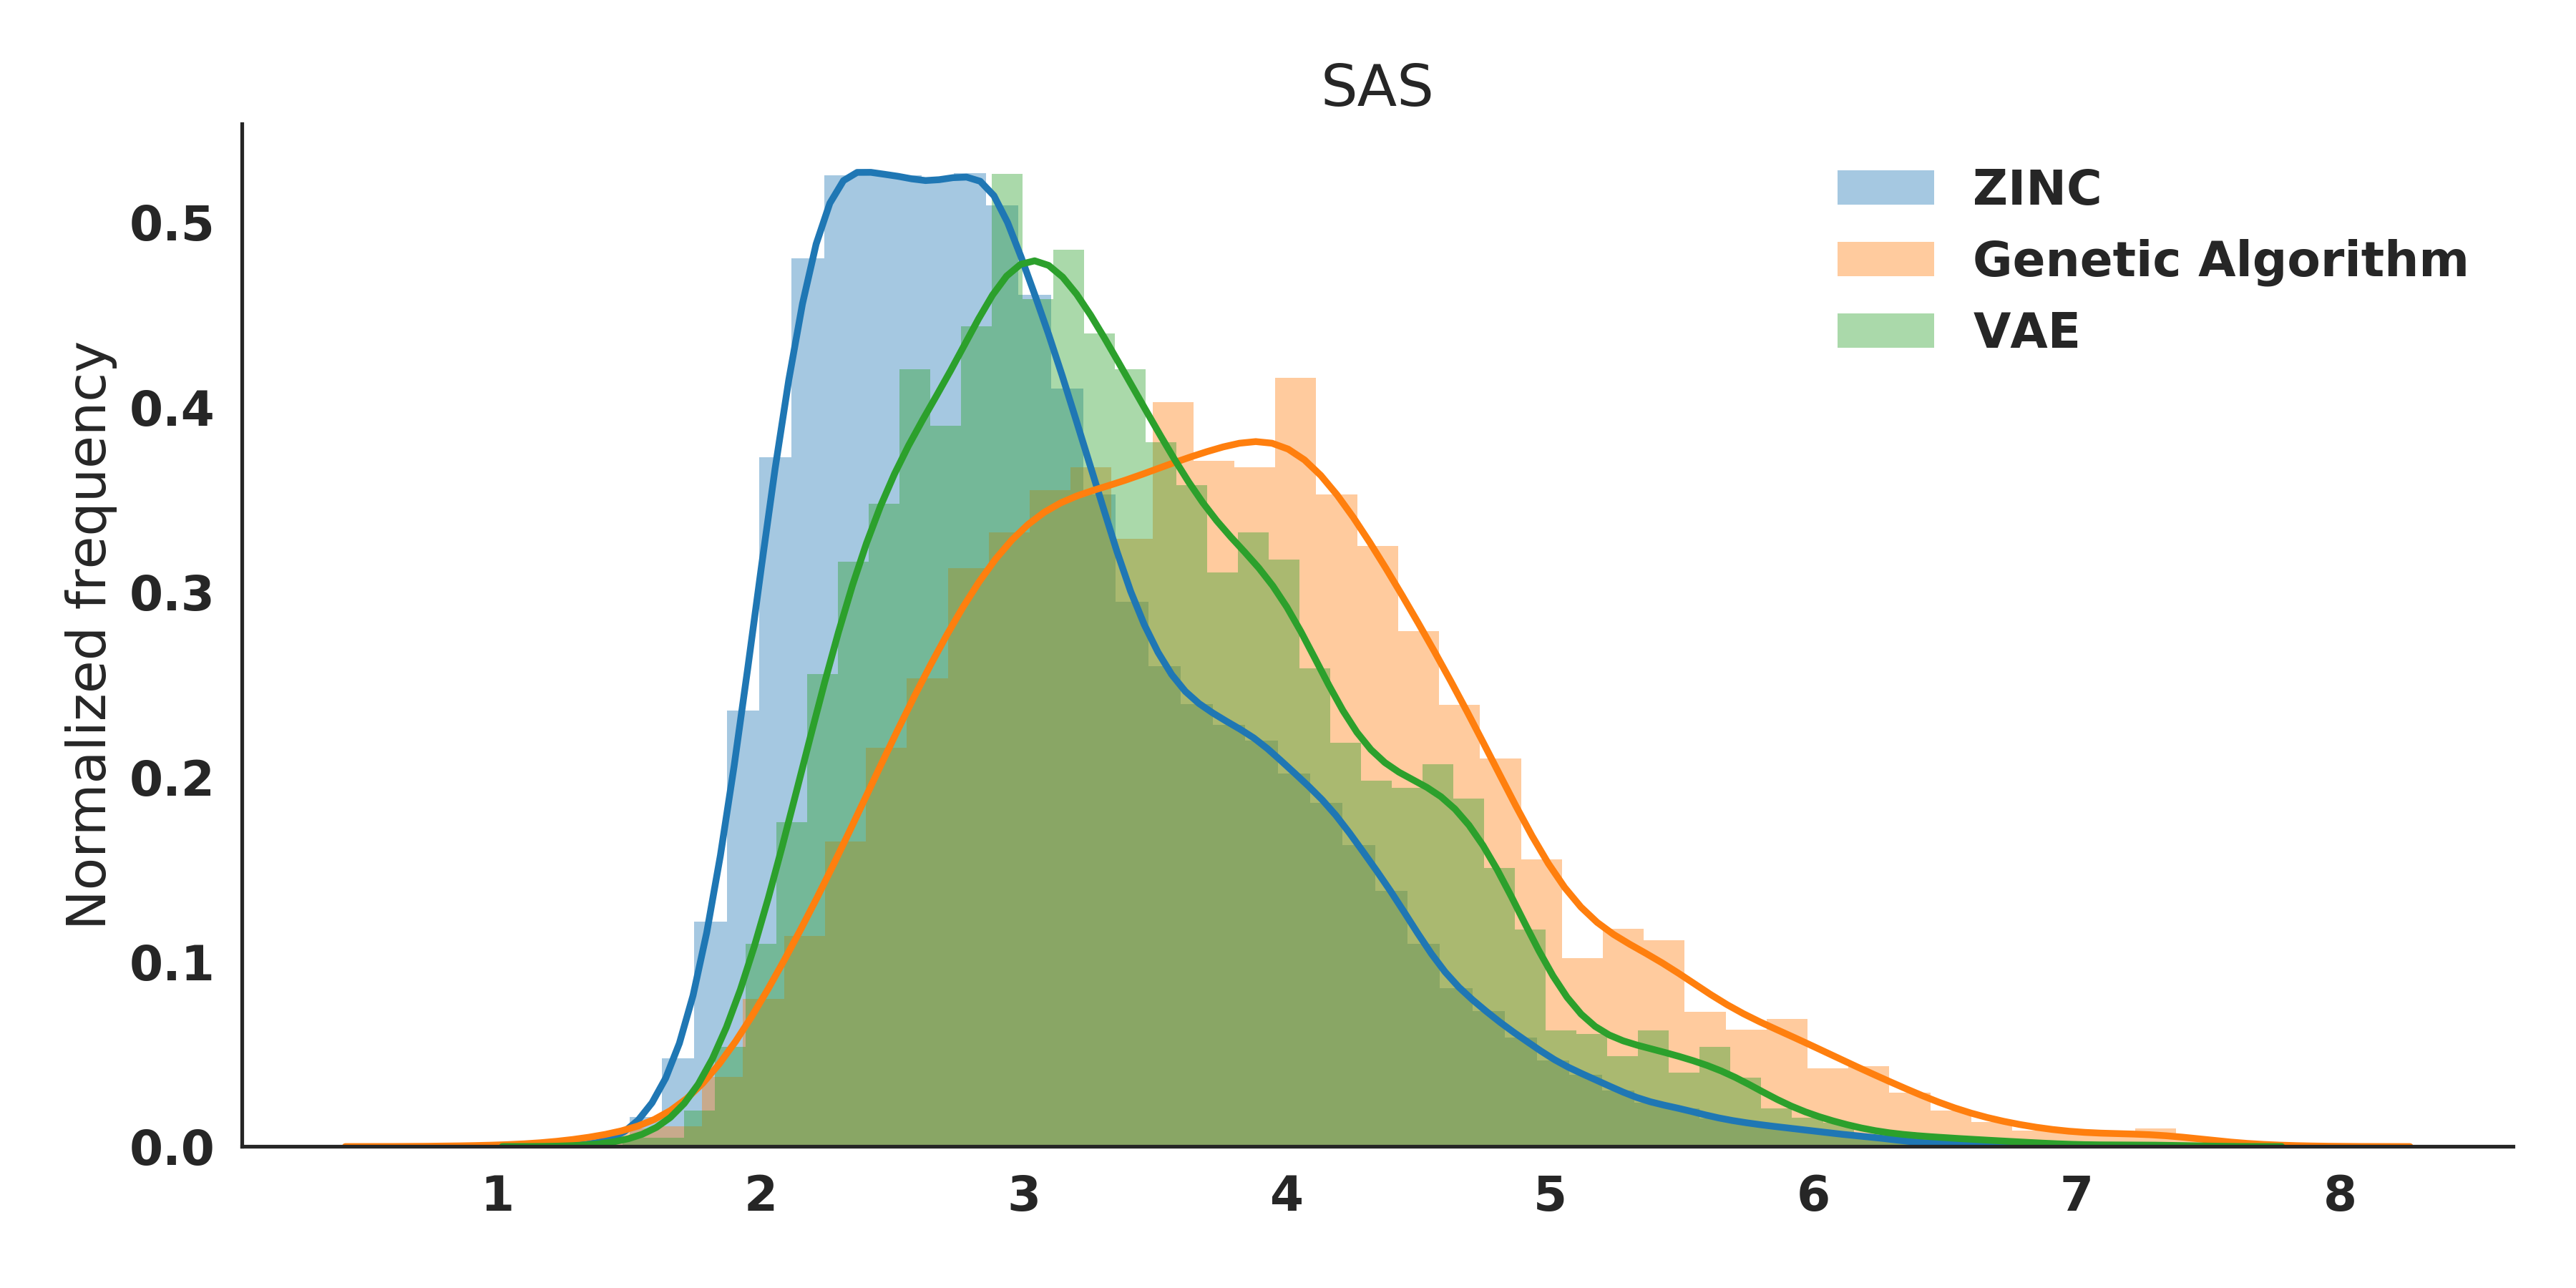
\includegraphics[width=0.3\columnwidth]{figures/SAS}
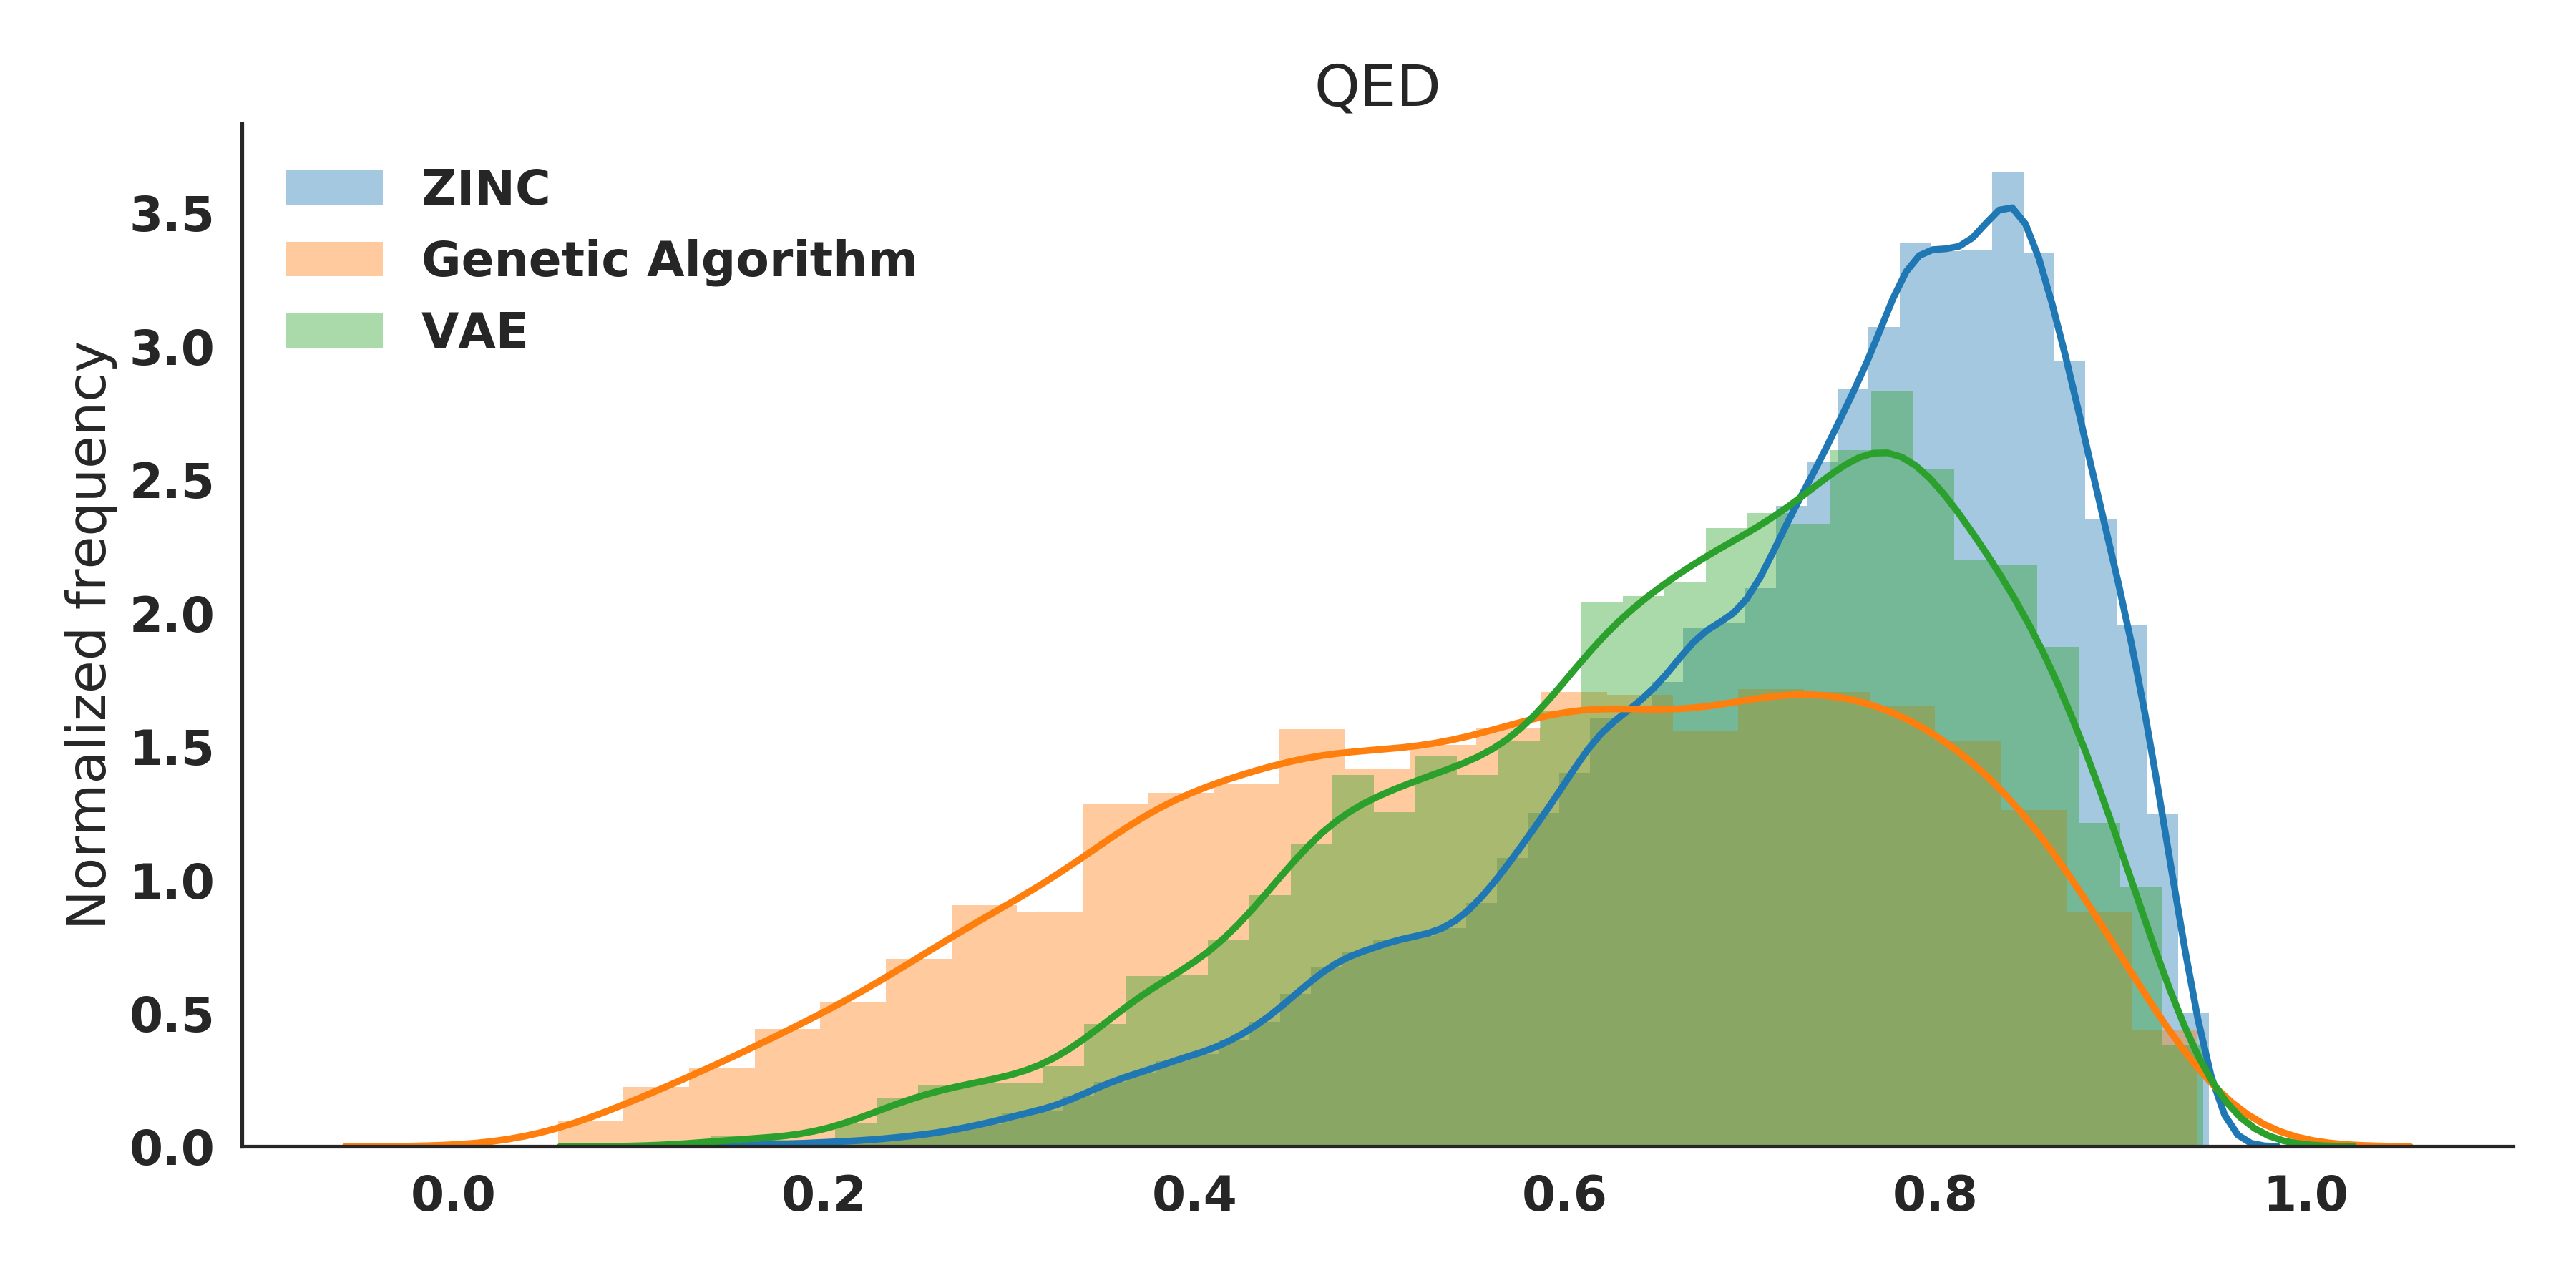
\includegraphics[width=0.3\columnwidth]{figures/QED}

\caption{Histograms and KDE plots of the distribution of properties utilized in the jointly trained autoencoder (LogP, SAS, QED). Used to further showcase results from Table 2. For each property we compare the distribution of the source data (ZINC), a generatic algorithm and the VAE.}
\label{fig:prop_dists}
\end{figure}


\begin{figure}
\centering
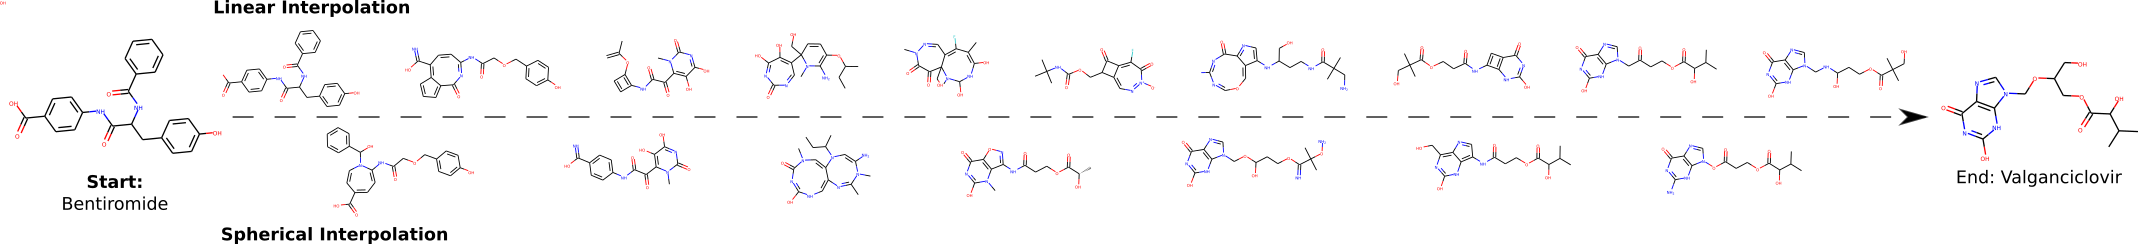
\includegraphics[width=\columnwidth]{figures/Slerp-lerp_compare}
\caption{Comparison of between linear and spherical interpolation paths between two randomly selected FDA approved drugs. A constant step size was used.}
\label{fig:interpol_1}
\end{figure}


\begin{figure}[h]
\centering
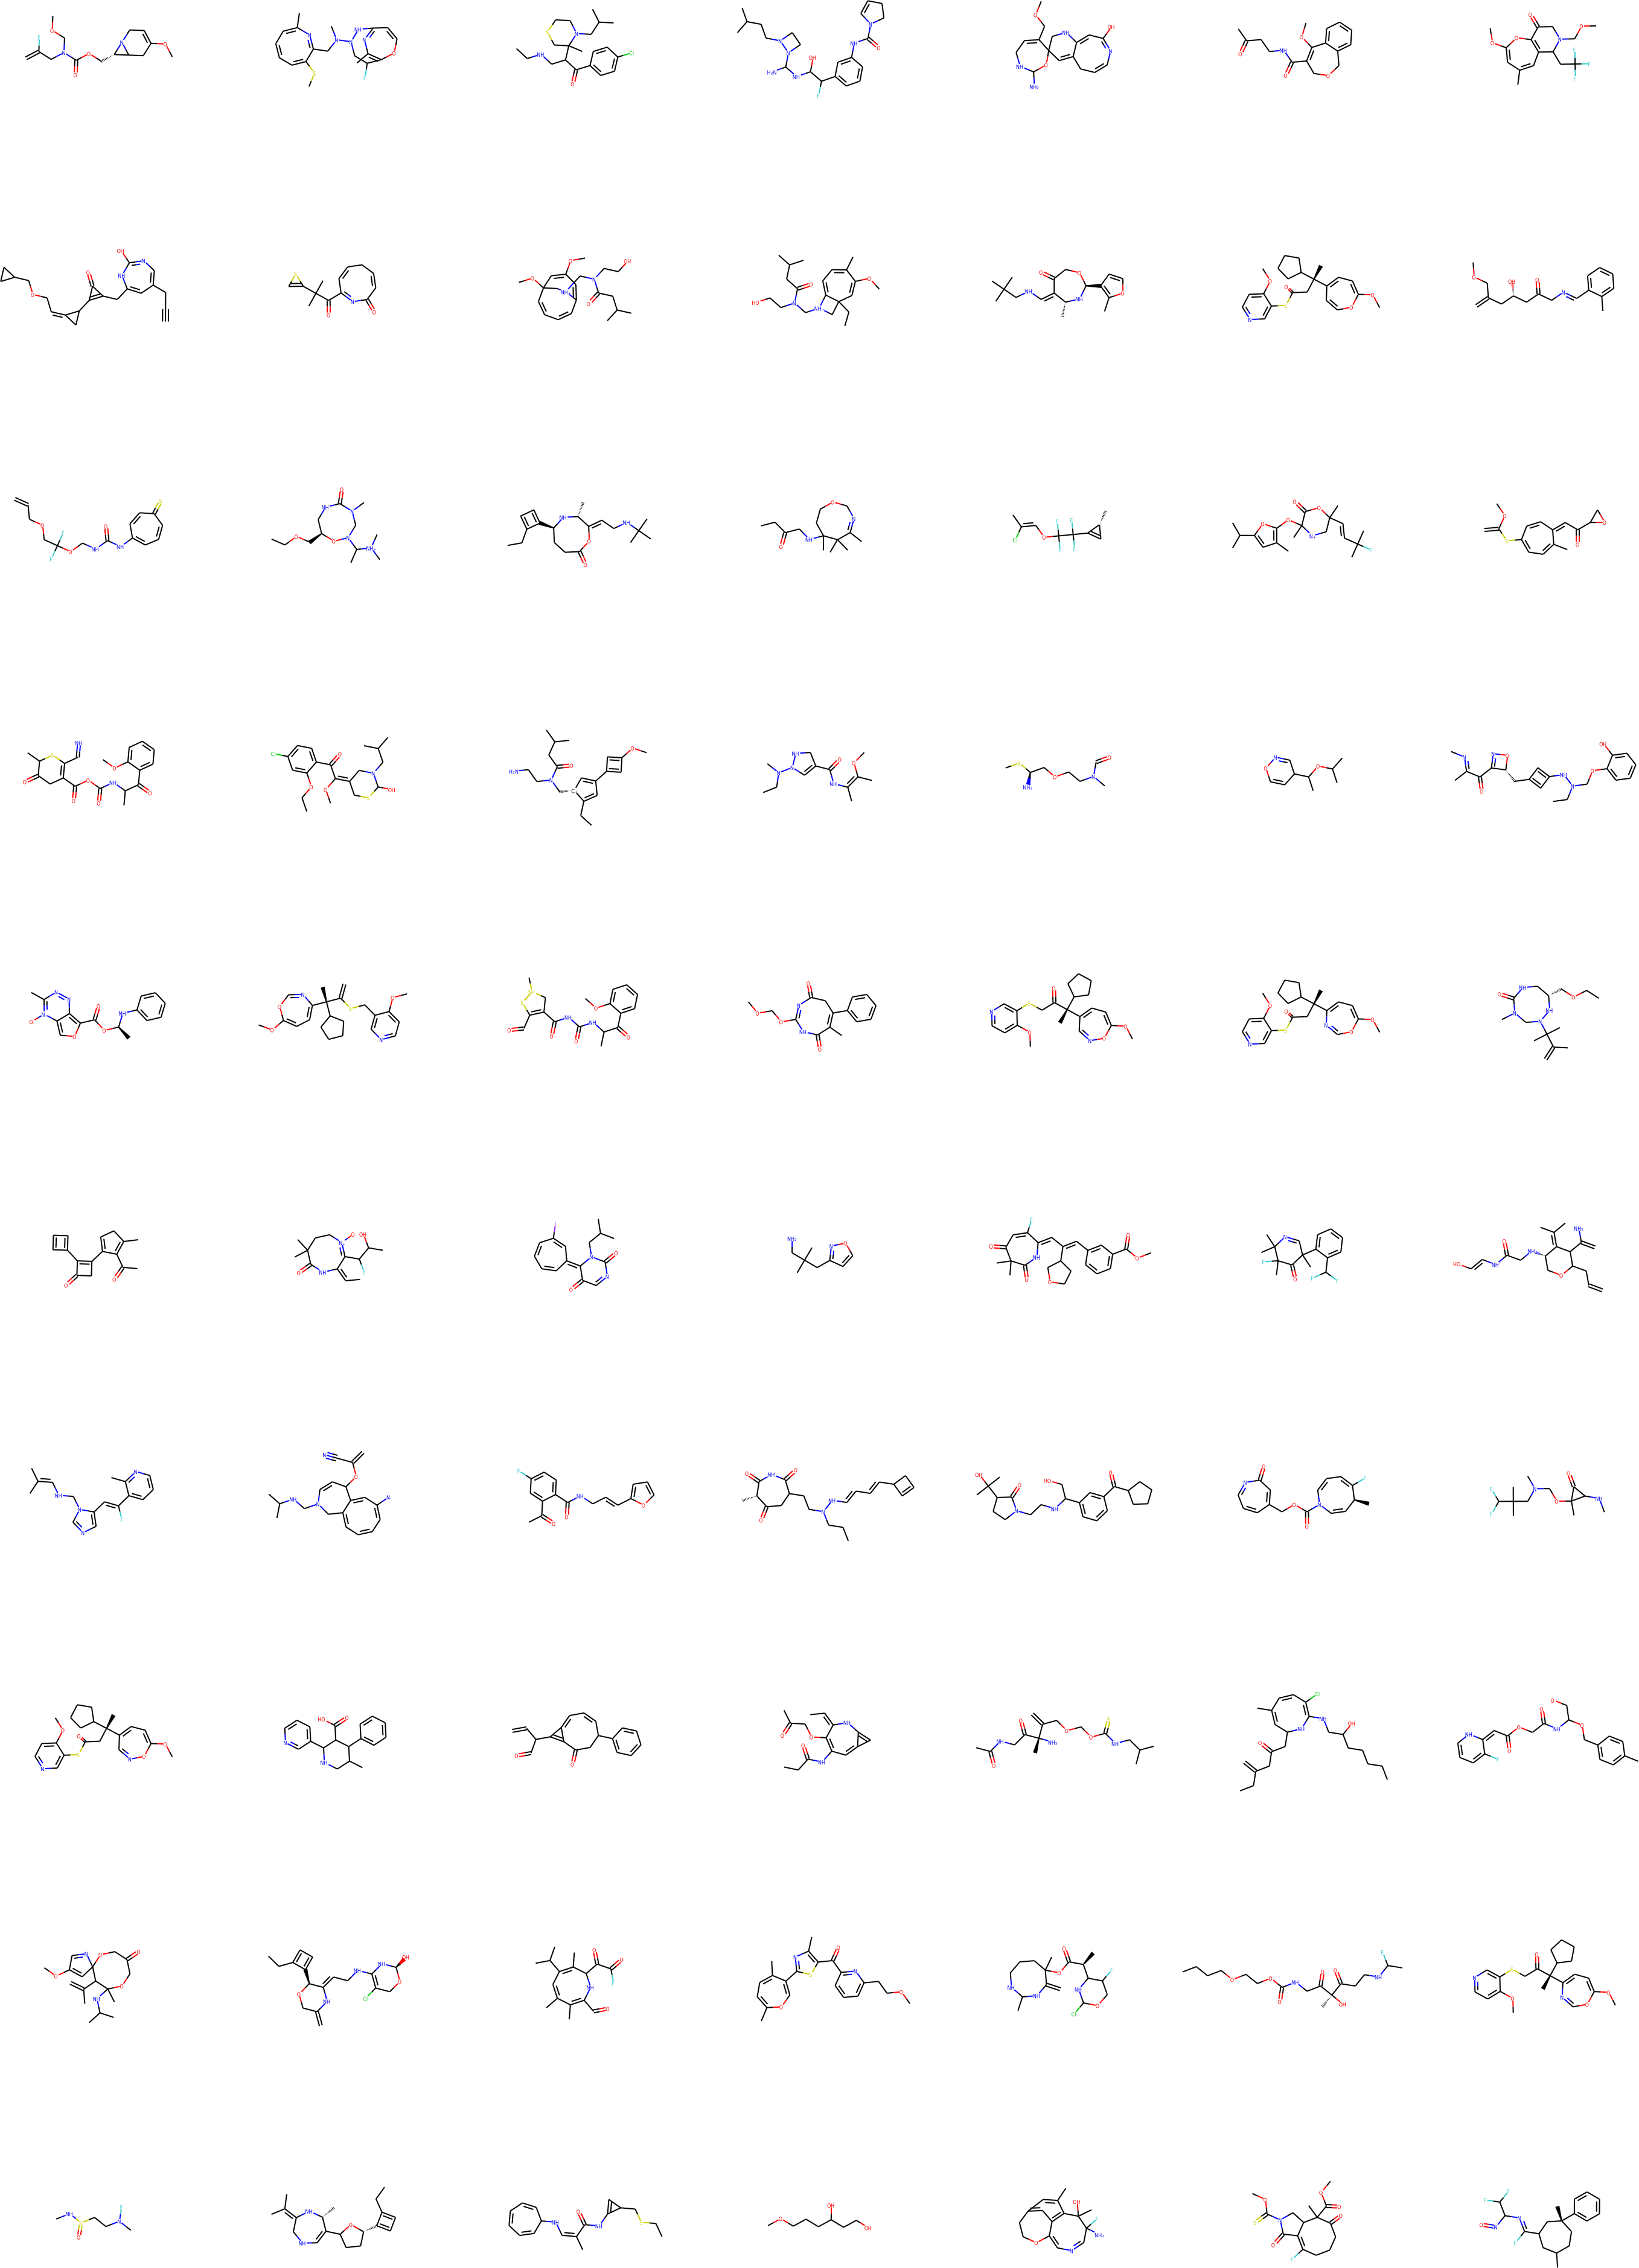
\includegraphics[width=0.9\columnwidth]{figures/VAE_random.png} 
\caption{Molecules decoded from randomly-sampled points in the latent space of the ZINC VAE.}
\label{fig:random_3}
\end{figure}







\end{document}
